\begin{section}{Conceptos}
En este apartado se describen algunos conceptos que se deben tener claros para entender la estructura y arquitectura de los componentes de VMware Cloud Foundation.
% En este apartado se describe la arquitectura de VMware Cloud Foundation y como estructura sus componentes\footnote{Se describen solo aquellos componentes que se utilizarán en el despliegue de Cloud Foundation.} internamente.

%%%%%%%%%%%%%%%%%%%%%%%%%%%%%%
% \iffalse
% En este apartado se explican aquellos conceptos de VMware Cloud Foundation necesarios para entender su funcionamiento, configuración y requisitos de la infraestructura previos al despliegue del servicio.
% \fi
%%%%%%%%%%%%%%%%%%%%%%%%%%%%%%%%


%% Workload Ddomains %&%&%%%%
%%%%%%%%%%%%%%%%%%%%%%%%%%%%
\begin{subsection}{Workload Domain}
Un Workload Domain (WD) representa un bloque de recursos dentro del SDDC, formado por recursos físicos y virtuales, gestionados por los componentes de VCF. En cada WD se despliegan instancias de los componentes de VCF para controlar el acceso y uso de los recursos virtuales y físicos, estableciendo, además, una capa de seguridad sobre el WD. Esto permite que los recursos de cada WD se gestionen de forma separada. La función de un WD consiste en separar flujos de trabajo para determinar que recursos se dedican a la realización de determinadas tareas.
% Un \textit{workload domain} consiste en una instancia lógica de un SDDC que abarca todos o parte de los recursos de uno o más clusters, cuya función es aislar el flujo de trabajo de un usuario, aplicación o un determinado tipo de tareas. Cada \textit{workload domain} se extiende sobre varios hosts con el hipervisor ESXi, y contiene sus propias instancias de VMware vCenter Server, VMware vSAN y VMware NSX-T. Así, esta arquitectura permite establecer políticas de control específicas para un \textit{workload domain} y otras comunes para todos o varios \textit{workload domains} y específicas para cada uno de ellos a la vez que se simplifica la complejidad de la infraestructura. Existen \underline{tres tipos} de \textit{workload domains} que permiten aislar las tareas de gestión de la infraestructura del resto de flujos de trabajo. 

%% MANAGEMENT DOMAIN
\begin{subsubsection}{Management Domain}
\label{subsubsec:domainManagement}
% Este \textit{workload domain} se crea y configura automáticamente durante el proceso de despliegue de una instancia de VMware Cloud Foundation.
El Management Domain es el primer WD que se crea dentro del SDDC cuando se despliega VCF. Su finalidad es alojar todos los componentes de VCF que gestionan el propio Management Domain y al resto de WDs. Inicialmente, se despliegan las siguientes VMs de cada componente:

\begin{itemize}
  \item Una VM de SDDC Manager.
  \item Una VM de VMware vCenter Server.
  \item Tres VMs de VMware NSX-T Manager Appliance.
  \item Dos VMs de VMware NSX-T Edge.
\end{itemize}
Al contener todas las instancias de los componentes dedicados a la gestión del SDDC, todas las tareas de administración suceden dentro de este WD. De esta forma, su ejecución está centralizada, es más segura y está mejor controlada, ya que lo hacen sobre un conjunto de recursos dedicados exclusivamente a ellas.
% El administrador gestiona los recursos del Management Domain, tanto hosts como instancias de los componentes, desde VMware vSphere Client, y VMware NSX-T Manager se encarga de controlar y mantener las redes virtuales del SDDC. Con VMware SDDC Manager, el administrador gestiona de forma centralizada los aspectos que afectan al ciclo de vida de todos los componentes del SDDC.


% Incluye las siguientes instancias: SDDC Manager, vCenter Server, una instancia de NSX Manager, tres instancias de NSX Controller, dos instancias de Platform Services Controller y tres instancias de vRealize Log Insight \cite{sddcComponents} [Fig. \ref{fig:componentsMNGDomain}].\\
% Cuando se \underline{despliega \textit{management domain} se crean y configuran} de forma automatizada por SDDC Manager las siguientes máquinas virtuales (VM) de cada componente de Cloud Foundation\footnote{Las características de cada máquina virtual se refieren a los requisitos mínimos}:
% \begin{itemize}
%     \item Una VM de \textbf{SDDC Manager}: 4 vCPU, 16 GB de memoria, 800 GB de almacenamiento.
%     \item Una VM de \textbf{vCenter Server}: 4 vCPU, 16 GB de memoria, 290 GB de almacenamiento.
%     \item Dos instancias de \textbf{Platform Services Controller} (cada una): 2 vCPU, 4 GB de memoria, 60 GB de almacenamiento.
%     \item Una VM de \textbf{NSX Manager}: 4 vCPU, 16 GB de memoria, 60 GB de almacenamiento.
%     \item Tres VM de \textbf{NSX Controller} (cada una): 4 vCPU, 4 GB de memoria, 28 GB de almacenamiento.
%     \item Tres VM de \textbf{vRealize Log Insight}: 4 vCPU, 8 GB de memoria, 250 GB de almacenamiento.
% \end{itemize}

% Para desplegar el \textit{management domain} se requieren las siguientes \underline{capacidades mínimas} en la infraestructura \cite{WDminRequierements}:
% \begin{itemize}
%     \item \textbf{Hosts}: 4
%     \item \textbf{CPU} por host: Dual-socket con 8 cores por socket, en sistemas All-Flash.
%     \item \textbf{Memoria} total: 192 GB
%     \item \textbf{Almacenamiento} por host: 16 GB para el dispositivo de arranque, un NVMe o SSD para la capa de caché, dos SSD o HDD para la capa de capacidad\footnote{En total se requieren 800 GB para este \textit{workload domain}.}.
%     \item \textbf{NICs} por host: Dos NICs de al menos 10 GbE y, opcionalmente un NIC 1GbE BMC.
% \end{itemize}

% \begin{figure}[h!]
%   \centering
%   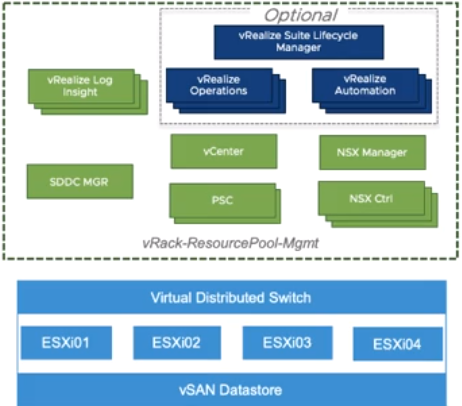
\includegraphics[width=0.5\textwidth]{imaxes/conceptosPrevios/componentsMANAGEDomain.png}
%   \caption{Componentes de \textit{management domain}}
%   \label{fig:componentsMNGDomain}
% \end{figure}
\end{subsubsection}

%% VIRTUAL INF. DOMAIN
\begin{subsubsection}{Virtual Infrastructure Domain (VI)}
\label{subsubsec:domainVI}
Este tipo de WD se crea manualmente y bajo demanda desde el Management Domain, para habilitar un entorno, cuyos recursos puedan ser usados por los usuarios mediante el despliegue de aplicaciones. Su configuración de hardware y lógica se especifican durante el proceso de creación, pudiendo establecer la cantidad de hosts, cantidad de almacenamiento, configuración de la red y políticas de rendimiento y disponibilidad, todo para satisfacer las necesidades del tipo de tareas que se van a realizar en él. Con la creación de un WD se generan las siguientes VMs:
% Con cada WD se genera un nuevo cluster de VMware vSphere que agrupa los nuevos recursos, aunque parte de sus componentes que se despliegan se controlan desde el Management Domain:
\begin{itemize}
  \item Una VM de VMware vCenter Server que se sitúa en el Management Domain.
  \item Tres VMs de VMware NSX-T Manager Appliance situadas en el Management Domain.
  \item Dos VMs de VMware NSX-T Edge.
\end{itemize}
Que ciertos componentes se sitúen en el Management Domain, permite separar las tareas de administración de un VI Domain de las aplicaciones y recursos de los usuarios, haciendo un entorno mejor organizado, más seguro y óptimo.

% El administrador gestiona los recursos del VI Domain desde VMware vSphere Client y la instancia de SDDC Manager situada en el Management Domain, y gestiona las redes virtuales del WD desde VMware NSX-T Manager situado también en el Management Domain. Los usuarios despliegan sus aplicaciones sobre los recursos de este WD, de esta forma, las tareas administrativas y las de consumo se ejecutan desde entornos separados.
% La diferencia entre un \textit{virtual infrastructure domain} y \textit{virtual desktop infrastructure domain} es que el segundo incorpora el producto VMware Horizon View que, resumiendo, permite desplegar escritorios virtuales. 
% Con cada nuevo \textit{virtual infrastructure domain} se crea un nuevo cluster vSphere en la infraestructura que agrupa todos los recursos que tiene asignados.\\
% Cuando se \underline{despliega un \textit{virtual infrastructure domain} se crean y configuran} de forma automatizada por el componente SDDC Manager las siguientes máquinas virtuales (VM) de cada componente de VMware Cloud Foundation\footnote{Las características de cada máquina virtual se refieren a los requisitos mínimos} 
%\cite{sddcComponents} [Fig. \ref{fig:compoVIdomain}]:
% \begin{itemize}
%     \item Una VM de \textbf{vCenter Server} en Management Domain: 8 vCPU, 24 GB de memoria, 500 GB de almacenamiento.
%     \item Una VM de \textbf{NSX Manager} en Management Domain: 4 vCPU, 16 GB de memoria, 60 GB de almacenamiento.
%     \item Tres VM de \textbf{NSX Controller} en el VI Domain creado (cada una):  4 vCPU, 4 GB de memoria, 28 GB de almacenamiento.
% \end{itemize}

% Por cada \textit{virtual infraestructure domain} que se despliega en la infraestructura, se requieren las siguientes capacidades mínimas\cite{WDminRequierements}:
% \begin{itemize}
%     \item \textbf{Hosts}: 3
%     \item \textbf{CPU}, \textbf{Memoria} y \textbf{Almacenamiento}: depende de los requisitos de las tareas que se vayan a desarrollar en este \textit{workload domain}.
%     \item \textbf{NICs} por servidor: Dos NICs de al menos 10 GbE y, opcionalmente un NIC 1 GbE BMC.
% \end{itemize}


 \end{subsubsection}

\end{subsection}
% \begin{figure}[h!]
%   \centering
%   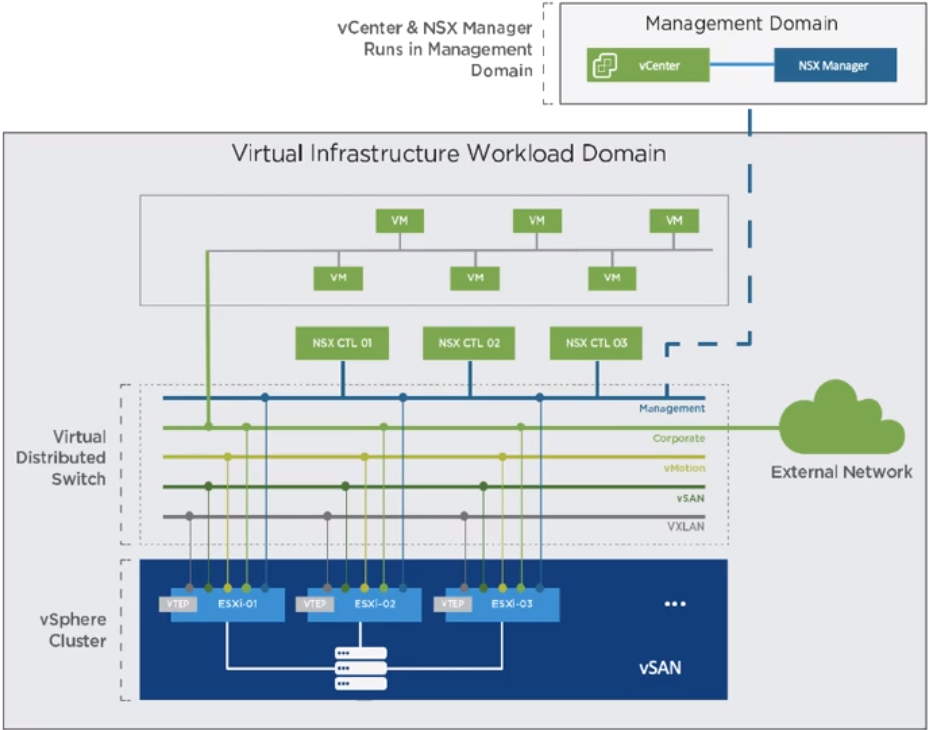
\includegraphics[width=0.5\textwidth]{imaxes/conceptosPrevios/networkArcVIDomain.png}
%   \caption{Componentes de \textit{virtual infrastructure domain}.}
%   \label{fig:compoVIdomain}
% \end{figure}
%\FloatBarrier

%&%%%%%%%%%%%%%%%%%%%%%%%%%%%%%%%%%%%%%%%%%%%%%%%%%%%%%%%%
%% ARQUITECTURA



\begin{subsection}{Arquitectura}
VMware proporciona dos posibles modelos de arquitectura diferentes. Se utiliza uno u otro dependiendo del tamaño de la infraestructura sobre la que se va a desplegar VCF, y con cada modelo, se determina la forma en la que se agruparán y administrarán los recursos del SDDC.

%%%%%%%%%%%%%%%%%%%%%
%%%%%%%%%%%%%%%%%%%%%%%%
%% ESTANDAR
\begin{subsubsection}{Modelo estándar}

Este modelo está pensado para entornos de tamaño medio/grande, con un mínimo de siete hosts. Está formado por un Management Domain y al menos un VI Domain. Esto implica que la ejecución de tareas dentro de un WD está limitada por los recursos que lo forman. Esto permite asignar roles a los recursos según las operaciones que se van a ejecutar sobre ellos, establecer un nivel de seguridad en cada WD y dedicar un conjunto de recursos a la ejecución de cierto tipo de operaciones. Así, el entorno es más eficiente, ya que se proporciona una forma de adecuar la configuración de los recursos de acuerdo con el uso que se va a hacer del servicio o servicios desplegados, minimizando además los cambios sobre la infraestructura física.
% esde el Management Domain se administra toda la infraestructura del SDDC y cada VI Domain existente, los cuales son creados bajo demanda desde el Management Domain y sus recursos se establecen según su finalidad. Un Management Domain puede gestionar hasta un máximo de de catorce VI Domain. 
%Cada \textit{virtual infrastructure domain} requiere tres hosts adicionales, es decir, un host solo puede pertenecer a un único \textit{workload domain}. 

\begin{figure}[h!]
  \centering
  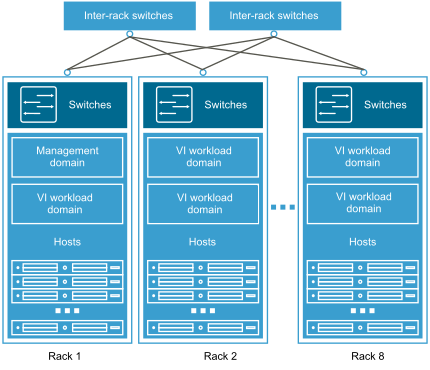
\includegraphics[width=0.6\textwidth]{imaxes/conceptosPrevios/arquitect_standarCF.png}
  \caption{Esquema del modelo de arquitectura estándar.}
  \label{fig:modelostandard}
\end{figure}

% \begin{figure}[h!]
%   \centering
%   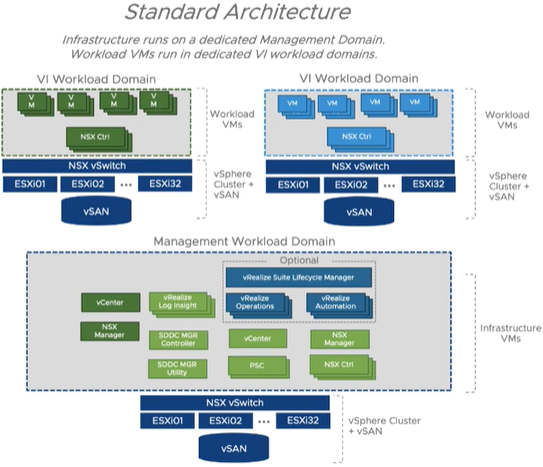
\includegraphics[width=0.6\textwidth]{imaxes/conceptosPrevios/standardArch.png}
%   \caption{Estructura de los componentes en una arquitectura estándar.}
%   \label{fig:standardarch}
% \end{figure}
\FloatBarrier
%%%%%%%%%%%%%%%%%%%%%
%%  CONSOLIDADO
\end{subsubsection}
\begin{subsubsection}{Modelo consolidado}
Este modelo está orientado a entornos de tamaño pequeño, con menos de siete hosts. Está formado por un único WD que cumple las funciones de un Management Domain y de un VI Domain, es decir, en él se colocan las instancias de los componentes dedicados a la gestión del SDDC\footnote{Se despliega la misma cantidad de instancias que en el Management Domain.} junto con las aplicaciones desplegadas para la realización de otro tipo de tareas. Así, a diferencia del modelo estándar, todas las operaciones se ejecutan dentro de un mismo entorno y sobre los mismos recursos. Internamente, las VMs se pueden colocar dentro de un grupo, llamado \textit{resource pools}, en el que se puede establecer un límite de uso de recursos.
Este modelo no aporta tantos beneficios como el modelo estándar, ya que todas las operaciones se realizan sobre los mismos recursos, y los niveles de control y seguridad son menores, por lo tanto su uso solo está recomendado para entornos de tamaño reducido.
% Dentro del cluster de VMware vSphere que se crea, las instancias pertenecientes a los componentes de administración del SDDC y las pertenecientes al trabajo de los usuarios, se colocan en \textit{resource pools} separados. Un \textit{resource pool} es un elemento de VMware vSphere que permite establecer unos límites de consumo de recursos sobre las instancias que se sitúan en su interior\cite{resourcePool}.

% Este modelo está pensado para desplegar VMware Cloud Foundation en entornos de tamaño pequeño, normalmente cuando hay menos de siete hosts, aunque también se puede utilizar en entornos más grandes con hasta 64 hosts. En este modelo los flujos de trabajo que corresponden al \textit{virtual infrastructure domain} y al \textit{management domain} en el despliegue estándar, están colocados dentro de un mismo \textit{workload domain} en un único cluster pero aislados gracias a que cada uno se coloca dentro de un \textit{resource pool} diferente, es decir, existe un cluster con varios \textit{resource pool}. El modelo consolidado se convierte en un modelo estándar cuando se añade un \textit{workload domain} al SDDC.[Fig. \ref{fig:modeloconsolidated}].

\begin{figure}[h!]
  \centering
  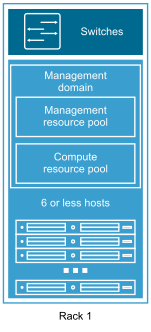
\includegraphics[width=0.25\textwidth]{imaxes/conceptosPrevios/modelConsolidated.png}
  \caption{Esquema del modelo de arquitectura consolidado.}
  \label{fig:modeloconsolidated}
\end{figure}

% \begin{figure}[h!]
%   \centering
%   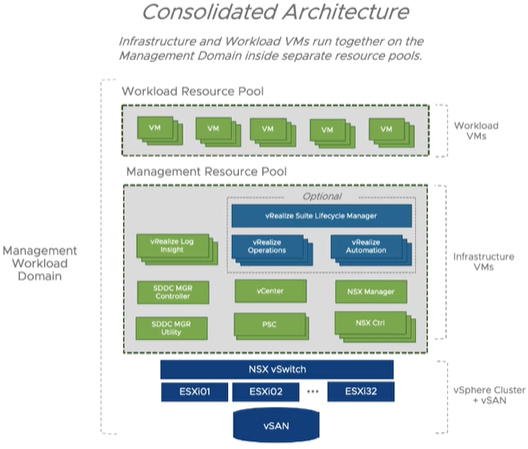
\includegraphics[width=0.6\textwidth]{imaxes/conceptosPrevios/consolidatedArch.png}
%   \caption{Estructura de los componentes de una arquitectura consolidado.}
%   \label{fig:consolidatedArch}
% \end{figure}
\FloatBarrier

\end{subsubsection}
\end{subsection}

\begin{subsection}{Clusters, zonas y distribución de un SDDC}

  Los recursos de un SDDC pueden estar distribuidos en diferentes localizaciones para proporcionar mayor disponibilidad y recuperación ante fallos. Estos recursos, se agrupan para formar una estructura que permite usar y gestionar los recursos disponibles de forma conjunta y dinámica.

\begin{subsubsection}{Availability Zone, Region y Cluster}
\begin{itemize}
  \item Availability Zone (AZ): se llama AZ a un conjunto de recursos físicos que forman una infraestructura independiente, es decir, cada una tiene su propia fuente de energía, su sistema de refrigeración, su sistema de seguridad y su red, no compartidos con otra AZ, para evitar la propagación de fallos hacia otras AZs. Cuando existen varias AZs, se pueden usar de forma que cuando ocurre un fallo en una de ellas la carga de trabajo se distribuye a una segunda AZ y, así, minimizar el tiempo de caída del servicio. Dentro de una AZ se alojan uno o más WDs.
  
  \item Region: se llama Region a un conjunto de AZs situadas en una misma ubicación, es decir, las AZs de una Region están situadas próximas entre sí. Estas AZs deben tener al menos una latencia de 5 ms entre ellas. Dentro de un SDDC pueden existir varias Regions pero estas se sitúan en ubicaciones más distantes, la latencia debe ser de al menos 150 ms. Esta estructura permite ofrecer los servicios de un SDDC en diferentes ubicaciones, a la vez que se aumenta su disponibilidad y recuperación ante fallos.
  
  \item Cluster: un cluster de VMware vSphere es una agrupación de hosts. A las instancias desplegadas sobre ellos, se les aplica una configuración de disponibilidad con el componente VMware vSphere, permitiendo determinar como se restablecen las instancias cuando ocurre un fallo dentro del cluster. Un cluster se sitúa dentro de un WD, por lo tanto, sus recursos estarán limitados por el alcance del WD. 
  %  Esta estructura permite acercar el servicio a ubicaciones separadas por grandes distancias. La arquitectura del modelo consolidado solo soporta una Region con una AZ, mientras que el modelo estándar permite desplegar múltiples Regions con múltiples AZs.
\end{itemize} 

\begin{figure}[h!]
  \centering
  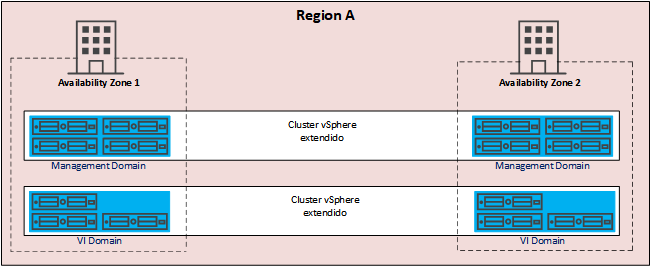
\includegraphics[width=0.8\textwidth]{imaxes/conceptosPrevios/AZRegionCluster.png}
  \caption{Ejemplo de un SDDC con dos Regions y una AZ en cada uno.}
  \label{fig:az-region-cluster}
\end{figure}
En la figura anterior se describe el esquema de un SDDC compuesto de una Region. Dentro de esta, existen dos AZ, AZ1 y AZ2. Cada una de las AZs contiene dos WD, un Management Domain desde donde se administra el SDDC, y un VI Domain donde se realizan las operaciones del SDDC. Como se mencionaba anteriormente, las instancias situadas en una AZ pueden migrar de una ubicación a otra en caso de fallo de los recursos físicos. Para ello, el WD donde se encuentran esas instancias debe estar extendido en las dos AZs. En la imagen, el Management Domain está formado por ocho hosts, repartidos en las AZs, los cuales están agrupados dentro del mismo cluster de VMware vSphere, por lo tanto, los componentes cuyas instancias estén situadas en este cluster se podrán migrar entre los 8 hosts. Estas migraciones se realizan en función de la configuración de disponibilidad establecida en los componentes VMware vSphere y VMware vSAN. Así, cuando los hosts de AZ1 sufren una caída, la AZ2 seguiría activa y las instancias situadas en AZ1 migrarían a AZ2 para continuar la disponibilidad del servicio, todo esto de forma automatizada, dinámica y transparente para el usuario. Lo mismo sucedería con el VI Domain\footnote{Se puede encontrar una descripción más detallada de esta estructura en el siguiente enlace \url{https://docs.vmware.com/en/VMware-Validated-Design/6.0/introducing-vmware-validated-design/GUID-661B1CE3-1F74-4E00-80F3-0F5EA39528CD.html}}.


\end{subsubsection}
% \begin{subsubsection}{Cluster y Resource Pool}
% Dentro de un \textit{workload domain} pueden existir varios clusters. Un cluster es una agrupación de hosts a cuyos recursos se les puede aplicar una una configuración de disponibilidad determinada con los componentes VMware vSphere High Availability y VMware vSphere Distributed Resource Scheduler para establecer como se restablece el servicio en caso de fallos en alguno de los hosts. Un cluster puede estar extendido en más de una AZ para que si una de las AZs falla, las aplicaciones que corrían en ella pueden ser migradas a otra AZ mejorando la disponibilidad del servicio. En un WD se despliegan dos clusters:
% \begin{itemize}
%   \item Management cluster: es el cluster que se crea al desplegar VMware Cloud Foundation. Contiene los componentes para administrar los recursos del WD.
%   \item Shared Edge and Workload Cluster: después del management cluster, este es el primero que se crea. Su finalidad es alojar las aplicaciones y cargas de trabajo de los usuarios dentro de un WD. Además contiene instancias de Vmware NSX-T para proporcionar sevicios de red.
% \end{itemize}

% Dentro de un cluster se pueden crear resource pools. Un \textit{resource pool} es una característica de VMware vSphere que permite abstraer un conjunto de recursos de un cluster estableciendo unos límites de capacidad que puede usar \cite{resourcePool}. Usar resource pools permite agrupar las VMs con una finalidad similar y controlar la cantidad de recursos del WD que esas VMs pueden consumir.

% Un SDDC puede estar distribuído en una o más \textit{Availability Zone} (AZ). Estas son zonas aisladas con infraestructuras independientes que evitan la propagación de fallos de hosts individuales a través de toda la infraestructura, cuantas más \textit{AZ} existan mayor disponibilidad tendrá el servicio. La latencia entre dos \textit{AZ} debe ser de 5 ms como máximo y la conexión de al menos 10 Gbit. Una \textit{Region} agrupa una o más \textit{AZ}s, con esto se da solución a la recuperación del servicio ante desastres. La latencia entre dos \textit{Region}s debe ser de 100 ms como máximo. El \underline{modelo consolidado} solo da soporte a una \textit{Region} con una \textit{AZ}, mientras que el \underline{modelo estándar} puede soportar múltiples \textit{Region} con múltiples \textit{AZ}.
% \end{subsubsection}
\end{subsection}

\end{section}

% \subsubsection{Clusters, zonas de disponibilidad y regiones}
% Un SDDC puede estar formado por uno o más clusters de distintos tipos. En el  \underline{modelo consolidado} la infraestructura está formada por un único cluster que incluye los servicios de gestión de VMware Cloud Foundation VMware vCenter Server, vSphere Update Manager, VMware NSX Manager, VMware NSX Controller y VMware vRealize Log Insight, los servicios de red necesarios para establecer conectividad en el entorno y las máquinas virtuales que los usuarios crean cuando aprovisionan sus recursos. Se aplican las mismas políticas de alta disponibilidad y gestión del ciclo de vida al flujo de trabajo de gestión del SDDC y al flujo de trabajo del usuario. En el \underline{modelo estándar} los distintos \textit{workload domain} se dividen en clusters que pueden ser de tres tipos:
%     \begin{itemize}
%         \item \textbf{Management Cluster}: se crea durante el despliegue de VMware Cloud Foundation y contiene el \textit{management domain}, desde aquí se gestiona el SDDC. Contiene los servicios de gestión mecionados anteriormente.
%         \item \textbf{Shared Edge and Compute Cluster}: es el primer cluster que se crea dentro de un \textit{virtual infrastructure domain} ya que puede haber más de un cluster. Este cluster contiene los servicios de red NSX del \textit{workload domain} y también puede contener el flujo de trabajo de los usuarios.
%         \item \textbf{Compute Cluster}: cluster adicional que se crea dentro de un \textit{virtual infraestructure domain}. Contiene el flujo de trabajo de los usuarios.
%     \end{itemize}
% Un SDDC puede estar distribuído en una o más \textit{Availability Zone} (AZ). Estas son zonas aisladas con infraestructuras independientes que evitan la propagación de fallos de hosts individuales a través de toda la infraestructura, cuantas más \textit{AZ} existan mayor disponibilidad tendrá el servicio. La latencia entre dos \textit{AZ} debe ser de 5 ms como máximo y la conexión de al menos 10 Gbit. Una \textit{Region} agrupa una o más \textit{AZ}s, con esto se da solución a la recuperación del servicio ante desastres. La latencia entre dos \textit{Region}s debe ser de 100 ms como máximo. El \underline{modelo consolidado} solo da soporte a una \textit{Region} con una \textit{AZ}, mientras que el \underline{modelo estándar} puede soportar múltiples \textit{Region}s con múltiples \textit{AZ}s.

%%%%%%%%%%%%%%%%%%%%%%%%%%%%%%%%%%%%%%%%%%%%
%%%%%%%%%%%%%%%%%%%%%%%%%%%%%%%%%%%%%%%%%%%%
%%%%%%%%%%%%%%%%%%%%%%%%%%%%%%%%%%%%%%%%%%%%
% \iffalse
% Un SDDC puede estar \underline{formado por múltiples clusters} que pueden ser de diferentes tipos con diferentes propósitos. Un cluster puede ocupar uno o más \textit{racks} dependiendo del nivel de escalabilidad que se requiera. Según su función, cada \textit{workload domain} se puede colocar en un cluster diferente para gestionar la alta disponibilidad y el ciclo de vida según sus necesidades. Un \underline{cluster puede ser de varios tipos}:
% \begin{itemize}
%     \item \textbf{Management Cluster}: Es aquel que contiene el \textit{management domain}, por lo tanto contiene las máquinas virtuales de los componentes que gestionan el SDDC. A este cluster solo deben acceder los administradores de la infraestructura.
%     \item \textbf{Shared Edge y Compute Cluster}: contiene el \textit{virtual infrastructure domain} con las máquinas virtuales de los usuarios y, además, incorpora servicios de NSX necesarios para comunicarse con redes externas y con otros \textit{workload domains}.
%     \item \textbf{Compute Cluster}: solo contiene el \textit{virtual infrastructure domain} con las máquinas virtuales de los usuarios.
%     \item \textbf{External Storage}: se centra en proveer almacenamiento de tipo NFS, iSCSI o Fiber Channel.
% \end{itemize}

% Un SDDC puede estar distribuído en una o más \underline{zonas de disponibilidad}. Estas son zonas aisladas que evitan la propagación de fallos de hosts individuales a través de toda la infraestructura, así, se puede entregar mayor disponibilidad de los recursos y servicios. A su vez, varias \underline{zonas de disponibilidad} se pueden agrupar en una \underline{región}, estos entornos separados por grandes distancias que permiten tener recuperación ante desastres [Fig. \ref{fig:AVRegiones}].\\

% \begin{figure}[h!]
%   \centering
%   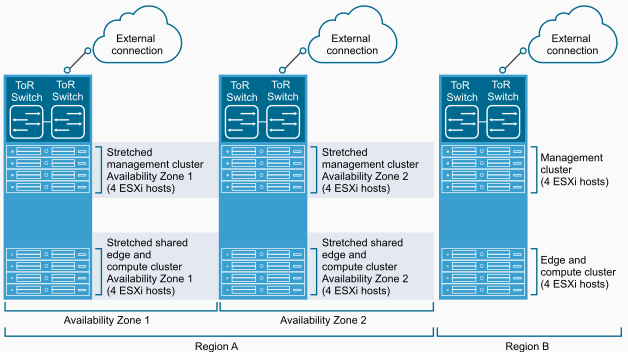
\includegraphics[width=0.95\textwidth]{imaxes/conceptosPrevios/zonasDispRegiones.png}
%   \caption{Una región contiene al menos una zona de disponibilidad.}
%   \label{fig:AVRegiones}
% \end{figure}
% \fi
%%%%%%%%%%%%%%%%%%%%%%%%%%%%%%%%%%%%%%%%%%%%%
%%%%%%%%%%%%%%%%%%%%%%%%%%%%%%%%%%%%%%%%%%%%%
%%%%%%%%%%%%%%%%%%%%%%%%%%%%%%%%%%%%%%%%%%%%%


